\chapter{Evaluation}
\label{ch: Verifikation}
Zur Evaluation der künstlichen neuronalen Netze wird eine \textit{Benchmark} durchgeführt. Hierbei wird anhand der in Abschnitt \ref{subsec: Entwickeltes neuronales Netz} beschriebenen Datensätze die \textit{Precision-Recall} Methode aus Abschnitt \ref{subsec: evaluation neuronaler netze} angewendet. Diese ist berücksichtigt Detektionen ab einem \textit{IoU}-Wert von~0,5.\\

 Weiterhin werden die Benchmarks auf dem integrierten Computer des ALFs und einem eingebetteten System ausgeführt. Als eingebettetes System wird ein \textit{Raspberry Pi 3 Model B} verwendet. Die Eckdaten des integrierten Computers sind in der entsprechenden Masterthesis dargestellt \cite{alf}.\\

Es ist keine geräteübergreifende Veränderung der Genauigkeit je Netz zu erwarten, da die Eingangsdaten und die Rechenoperationen identisch sind. Jedoch können so die Bearbeitungszeiten pro Bild für unterschiedliche Hardwareplattformen verglichen werden. Eine präzise Auflistung aller gemessenen Analysezeiten ist in Tabelle \ref{fig: zeitentab} präsentiert. \\

Insgesamt werden für die Benchmark 12755 Bilder von Personen aus dem Trainingsdatensatz entnommen, da der eigentliche Testdatensatz des \textit{COCO}-Datensatzes keine grundwahren Labels enthält. Die Unterteilung des Datensatzes in Trainings- und Testdaten geschah vor dem Training. Andernfalls würde ein Netz während der Benchmark mit bereits bekannten Trainingsdaten rechnen. Dies würde das Testergebnis verfälschen. \\
 

Der im Grundlagenabschnitt \ref{subsec: evaluation neuronaler netze} beschriebene \textit{mAP}-Wert wird häufig auf Objekterkennungssystemen mit multiplen Klassen angewendet. Die hier entwickelte Personenerkennung soll jedoch lediglich die Klasse \textit{Person} erkennen. Somit ist der \textit{mAP}-Wert in diesem Fall der Mittelwert eines Messwerts und kann als Integral der \textit{Precision-Recall}-Kurve angesehen werden. Im Verlauf der Evaluation der angewendeten Systeme wird mithilfe einer Berechnungssoftware jeweils der \textit{mAP}-Wert berechnet.
 
\section{Präsentation der Messergebnisse} 

Als Vergleich analysiert jedes Netz auch den eigenen Datensatz. So kann die Performance am Einsatzort des ALFs an der Hochschule Bochum evaluiert werden. Jedes Bild wird für die verwendeten, neuronalen Netze auf eine Pixelgröße von $300 \times 300$ skaliert. Für die Evaluation des \textit{HOG-SVM} Systems wird eine höhere Auflösung gewählt. Hierbei wird eine Seite des Bildes softwareseitig auf 400 Pixel begrenzt.

\subsection{Test der einzelnen Architekturen}

Die Kombination aus \textit{HOG} und \textit{SVM} erreicht in der Benchmark die in Abbildung \ref{fig: hog1} präsentierten Ergebnisse. Der \textit{mAP}-Wert liegt für den eigenen Datensatz bei 0,16 und für den \textit{COCO}-Datensatz bei 0,07.\\


\begin{figure}[H]
	\centering
	\begin{tikzpicture}[
	]
	\begin{axis}[
	width=12cm,
	height=7cm,
	axis y line*=left,
	ticklabel style={% gilt für x und y
		/pgf/number format/.cd,
		use comma,% Komma als Dezimaltrenner
		1000 sep = {}% keine Tausendertrennung 
	},
	xlabel={$\text{Recall } \textit{r(t)}$},
	ylabel={$\text{Precision } \textit{p(t)}$},
	axis x line*=bottom,
	xmin=0, xmax=0.3, 
	ymin=0, ymax=0.3,
	%every axis plot/.append style={line width=1.0pt}
	legend pos=north east,
	]
	
	\addlegendentry{Eigener Datensatz}; % legende1
	\addplot[gray, line width=0.8pt]  table [x=Step,y=Value,col sep=comma] from {Bilder/hog.csv};
	\addplot[black, line width=0.8pt]  table [x=Step,y=Value,col sep=comma] from {Bilder/hogcoco.csv};
	\addlegendimage{/pgfplots/refstyle=plotbrr};				
	\addlegendentry{\textit{COCO}-Datensatz} ;%legende 2;
	%\addlegendentry{plot 1}
	\end{axis}
	\end{tikzpicture}
	\caption{\textit{Precision-Recall}-Kurven des \textit{SSD MobileNet V2} Netz. Die schwarze Kurve beschreibt die Analyse durch den \textit{COCO}-Datensatz. Der Test mithilfe des eigenen Datensatz wir durch die graue Kurve präsentiert. https://github.com/kaka-lin/object-detection}
	\label{fig: ssdmobilenetv2}
\end{figure}





 Die eingetragenen \textit{Bounding Boxes} fallen bei der Durchsicht der Ergebnisse durch ihre große Fläche im Hinblick auf die zu erkennenden Personen auf. Dies lässt sich auf die Größe der Zellen zurückführen, da die Ausbreitung der \textit{Bounding Box} davon abhängig ist.\\
 
 Derartige Erkennungen führen zu einem kleinen \textit{IoU}-Wert und gehen somit negativ in der Bewertung ein. Der Versuch die Zellgröße zu reduzieren, wirkte sich jedoch ebenfalls negativ auf die Ergebnisse der Personenerkennung aus. Mit den entsprechenden Optimierungen wurden die \textit{Precision-Recall} Werte für dieses System maximiert. Diese sind in Abbildung \ref{fig: hog1} dargestellt.\\
	\begin{figure}[H]
	\centering
	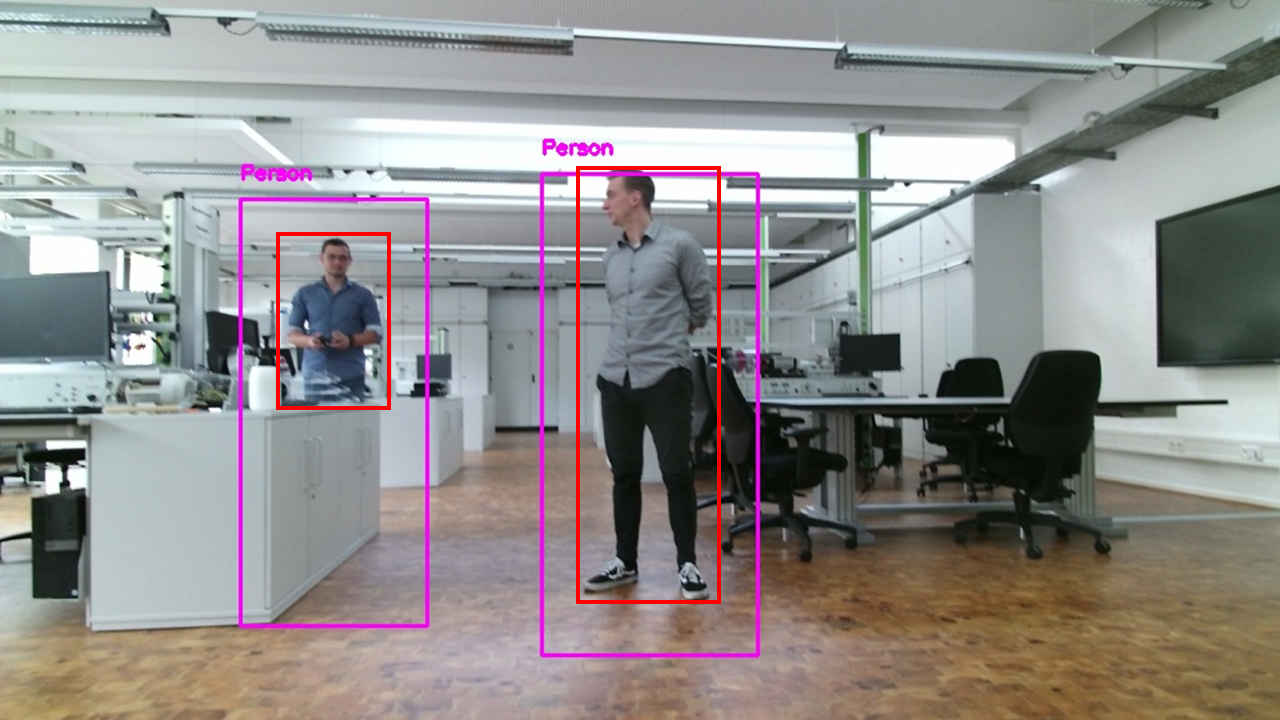
\includegraphics[width=1\textwidth]{Bilder/iouhog.png}
	\caption{Personenerkennung durch die \textit{HOG-SVM} Methode. Die grundwahren \textit{Bounding Boxes} sind in roter Farbe dargestellt. Durch das Netz extrahierte Begrenzungsrahmen werden durch pinke Rechtecke verdeutlicht.}
	\label{fig: hogiou}
\end{figure}

In Abbildung \ref{fig: hogiou} sind sowohl die grundwahren \textit{Bounding Boxes} in roter, sowie die durch die \textit{HOG-SVM} Methode ausgegebenen Begrenzungsrahmen in pinker Farbe gezeigt. Es ist zu erkennen, dass sich die extrahierten \textit{Bounding Boxes} im Vergleich zu den grundwahren unterscheiden.\\

 Vermutlich markiert das System bei der linken Person den vollständigen Körper aufgrund der Schranktüren, die unter der Person zu sehen sind. Diese erzeugen vertikal verlaufende Gradienten, wie auch die Beine einer Person.

\begin{figure}[H]
	\centering
	\begin{tikzpicture}[
	]
	\begin{axis}[
	width=12cm,
	height=7cm,
	axis y line*=left,
	ticklabel style={% gilt für x und y
		/pgf/number format/.cd,
		use comma,% Komma als Dezimaltrenner
		1000 sep = {}% keine Tausendertrennung 
	},
	xlabel={$\text{Recall } \textit{r(t)}$},
	ylabel={$\text{Precision } \textit{p(t)}$},
	axis x line*=bottom,
	xmin=0, xmax=1, 
	ymin=0, ymax=1.2,
	%every axis plot/.append style={line width=1.0pt}
	legend pos=north east,
	]
	
	\addlegendentry{Eigener Datensatz}; % legende1
	\addplot[gray, line width=0.8pt]  table [x=Step,y=Value,col sep=comma] from {Bilder/cocossdmobilenetv1tflite.csv};
	\addplot[black, line width=0.8pt]  table [x=Step,y=Value,col sep=comma] from {Bilder/cocossdmobilenetv1cocotest.csv};
	\addlegendimage{/pgfplots/refstyle=plotbrr};				
	\addlegendentry{\textit{COCO}-Datensatz} ;%legende 2;
	%\addlegendentry{plot 1}
	\end{axis}
	\end{tikzpicture}
	\caption{Gegenüberstellung der \textit{Precision} und \textit{Recall} Kurven eines quantisierten \textit{Tensorflow Lite SSD MobileNet V1} Netzes. Durch die schwarze Kurve wird das Testergebnis durch den \textit{COCO}-Datensatz gezeigt. Die graue Kurve zeigt das \textit{Precision} und \textit{Recall} Verhältnis für die Analyse des eigenen Datensatzes. Tensorflow starter}
	\label{fig: ssdmobilenetv1}
\end{figure}


Eine deutliche Steigerung hinsichtlich der Genauigkeit im Vergleich zur \textit{HOG-SVM} Methode wird durch das quantisierte \textit{MobileNet V1 SSD} Netz erreicht. Die Berechnung des Integrals der \textit{Precision-Recall} Kurve ergab für den eigenen Datensatz einen Wert von 0,68 und für den \textit{COCO}-Datensatz 0,46. Dieses Netz ist in der Lage 90 verschiedene Klassen zu erkennen. Hierbei nimmt das Netz jedoch lediglich 4 MB Speicherplatz ein.\\


\begin{figure}[H]
	\centering
	\begin{tikzpicture}[
	]
	\begin{axis}[
	width=12cm,
	height=7cm,
	axis y line*=left,
	ticklabel style={% gilt für x und y
		/pgf/number format/.cd,
		use comma,% Komma als Dezimaltrenner
		1000 sep = {}% keine Tausendertrennung 
	},
	xlabel={$\text{Recall } \textit{r(t)}$},
	ylabel={$\text{Precision } \textit{p(t)}$},
	axis x line*=bottom,
	xmin=0, xmax=1, 
	ymin=0, ymax=1.2,
	%every axis plot/.append style={line width=1.0pt}
	legend pos=north east,
	legend cell align={left},
	]
	
	\addlegendentry{\footnotesize Eigener Datensatz}; % legende1
	\addplot[gray, line width=0.8pt]  table [x=Step,y=Value,col sep=comma] from {Bilder/ownssdmobilenetv1.csv};
	\addplot[line width=0.8pt]  table [x=Step,y=Value,col sep=comma] from {Bilder/ownnetv1coco.csv};
	\addlegendimage{/pgfplots/refstyle=plotbrr};				
	\addlegendentry{\footnotesize \textit{COCO}-Datensatz} ;%legende 2;
	%\addlegendentry{plot 1}
	\end{axis}
	\end{tikzpicture}
	\caption{\textit{Precision-Recall}-Kurven des entwickelten \textit{MobileNet V1 SSD} Netzes.}
	\label{fig: ownnetv1}
\end{figure}


Das in Abbildung \ref{fig: ownnetv1} gezeigte \textit{MobileNet V1 SSD} Netz ist darauf trainiert, lediglich Personen zu erkennen. Die dargestellte Architektur weist einen \textit{mAP}-Wert von 0,79 für den eigenen Datensatz und 0,56 für den \textit{COCO}-Datensatz auf. \\

Bereits jetzt lässt sich eine Tendenz bezüglich der Messergebnisse je Datensatz erkennen. Die Objekterkennungssysteme erreichen bei dem Test auf den \textit{COCO}-Datensatz niedrige Messwerte im Vergleich zu dem Test auf den eigenen Datensatz. Hiermit bestätigt sich die These aus Abschnitt \ref{subsec: Entwickeltes neuronales Netz}, in der die Schwierigkeit der Personenerkennung auf den \textit{COCO}-Datensatz beschrieben wird.


\begin{figure}[H]
	\centering
	\begin{tikzpicture}[
	]
	\begin{axis}[
	width=12cm,
	height=7cm,
	axis y line*=left,
	ticklabel style={% gilt für x und y
		/pgf/number format/.cd,
		use comma,% Komma als Dezimaltrenner
		1000 sep = {}% keine Tausendertrennung 
	},
	xlabel={$\text{Recall } \textit{r(t)}$},
	ylabel={$\text{Precision } \textit{p(t)}$},
	axis x line*=bottom,
	xmin=0, xmax=1, 
	ymin=0, ymax=1.2,
	%every axis plot/.append style={line width=1.0pt}
	legend pos=north east,
	]
	
	\addlegendentry{Eigener Datensatz}; % legende1
	\addplot[gray, line width=0.8pt]  table [x=Step,y=Value,col sep=comma] from {Bilder/ownnetv2.csv};
	\addplot[line width=0.8pt]  table [x=Step,y=Value,col sep=comma] from {Bilder/ownnetv2coco.csv};
	
	\addlegendimage{/pgfplots/refstyle=plotbrr};				
	\addlegendentry{\textit{COCO}-Datensatz} ;%legende 2;
	%\addlegendentry{plot 1}
	\end{axis}
	\end{tikzpicture}
	\caption{\textit{Precision-Recall}-Kurven des enwtickelten \textit{SSD MobileNet V2} Netz.}
	\label{fig: ssdmobilenetv2}
\end{figure}


In Darstellung \ref{fig: ownnetv2} werden die \textit{Precision-Recall} Kurven eines \textit{MobileNet V2 SSD} gezeigt. Das Verhaltensmuster dieses Netzes ist ebenfalls auf eine Personenerkennung beschränkt, um enthaltene Parameter und den damit verbundenen Speicherplatz zu reduzieren.\\

Die \textit{mAP}-Werte liegen bei 0,78 für den eigenen Datensatz und 0,54 für den \textit{COCO}-Datensatz. Insgesamt weist das dargestellte, modifizierte \textit{MobileNet V2 SSD} Netz leichte, negative Abweichungen der \textit{Recall}-Werte im Vergleich zur zuvor präsentierten \textit{MobileNet V1 SSD} Architektur auf. Dies entspricht jedoch den Erwartungen aus dem Abschnitt \ref{subsec: Auswahl und Training der verwendeten neuronalen Netze}.


\begin{figure}[H]
	\centering
	\begin{tikzpicture}[
	]
	\begin{axis}[
	width=12cm,
	height=7cm,
	axis y line*=left,
	ticklabel style={% gilt für x und y
		/pgf/number format/.cd,
		use comma,% Komma als Dezimaltrenner
		1000 sep = {}% keine Tausendertrennung 
	},
	xlabel={$\text{Recall } \textit{r(t)}$},
	ylabel={$\text{Precision } \textit{p(t)}$},
	axis x line*=bottom,
	xmin=0, xmax=1, 
	ymin=0, ymax=1.2,
	%every axis plot/.append style={line width=1.0pt}
	legend pos=north east,
	]
	
	\addlegendentry{Eigener Datensatz}; % legende1
	\addplot[gray, line width=0.8pt]  table [x=Step,y=Value,col sep=comma] from {Bilder/ssdmobilenetv2tflite.csv};
	\addplot[black, line width=0.8pt]  table [x=Step,y=Value,col sep=comma] from {Bilder/ssdmobilenetv2tflitecoco.csv};
	\addlegendimage{/pgfplots/refstyle=plotbrr};				
	\addlegendentry{\textit{COCO}-Datensatz} ;%legende 2;
	%\addlegendentry{plot 1}
	\end{axis}
	\end{tikzpicture}
	\caption{\textit{Precision-Recall}-Kurven eines \textit{SSD MobileNet V2} Netz \cite{ssdv2}. }
	\label{fig: ssdmobilenetv2}
\end{figure}


Abbildung \ref{fig: ssdmobilenetv2} zeigt die \textit{Precision} und \textit{Recall} Kurve einer \textit{MobileNet V2 SSDLite} Architektur. Auffällig hierbei ist die hohe Genauigkeit $p(t)$ bei dem Test auf den \textit{COCO}-Datensatz. Im Vergleich zu den anderen untersuchten Architekturen liegt diese für niedrige \textit{Recall}-Werte nahe eins.\\

 Für die Anwendung auf den eigenen Datensatz erreicht die \textit{MobileNet V2 SSDLite} Architektur eine mittlere Durchschnittsgenauigkeit von 0,77. Angewendet auf den \textit{COCO}-Datensatz liegt der Wert bei 0,54. Somit konnten  keine nennenswerten Unterschiede im Bezug auf die Genauigkeit der beiden Detektoren \textit{SSD} und \textit{SSDLite} festgestellt werden. \\
 
 Die \textit{Precision-Recall}-Kurven der modifizierten \textit{MobileNet V2 SSDLite} Architektur sind in der Grafik \ref{fig: ownnetv2ssdlite} abgebildet. Dieses Netz wurde lediglich auf die Erkennung von Personen trainiert. Das Resultat für die Anwendung auf den eigenen Datensatz zeigt einen \textit{mAP}-Wert von 0,74. Einen \textit{mAP}-Wert von 0,47 ergab der Test auf den \textit{COCO}-Datensatz.\\ 

 

\begin{figure}[H]
	\centering
	\begin{tikzpicture}[
	]
	\begin{axis}[
	width=12cm,
	height=7cm,
	axis y line*=left,
	ticklabel style={% gilt für x und y
		/pgf/number format/.cd,
		use comma,% Komma als Dezimaltrenner
		1000 sep = {}% keine Tausendertrennung 
	},
	xlabel={$\text{Recall } \textit{r(t)}$},
	ylabel={$\text{Precision } \textit{p(t)}$},
	axis x line*=bottom,
	xmin=0, xmax=1, 
	ymin=0, ymax=1.2,
	%every axis plot/.append style={line width=1.0pt}
	legend pos=north east,
	legend cell align={left},
	]
	
	\addlegendentry{\footnotesize Eigener Datensatz}; % legende1
	\addplot[gray, line width=0.8pt]  table [x=Step,y=Value,col sep=comma] from {Bilder/ownnetv2ssdlite.csv};
	\addplot[line width=0.8pt]  table [x=Step,y=Value,col sep=comma] from {Bilder/ownnetv2ssdlitecoco.csv};
	
	\addlegendimage{/pgfplots/refstyle=plotbrr};				
	\addlegendentry{\footnotesize \textit{COCO}-Datensatz} ;%legende 2;
	%\addlegendentry{plot 1}
	\end{axis}
	\end{tikzpicture}
	\caption{Darstellung der \textit{Precision-Recall}-Verläufe des enwtickelten \textit{MobileNet V2 SSDLite} Netz.}
	\label{fig: ownnetv2ssdlite}
\end{figure}

 
  


Ein Beispiel der Personenerkennung durch das modifizierte \textit{MobileNet V2 SSDLite} Netz ist in Abbildung \ref{fig: ownnetiou} dargestellt. Das Bild stammt aus dem eigenen Datensatz und zeigt eine kniende Person im Labor für Antriebstechnik der Hochschule Bochum. Die Person wird durch das Netz mithilfe einer pinken \textit{Bounding Box} eingerahmt.\\
	\begin{figure}[H]
	\centering
	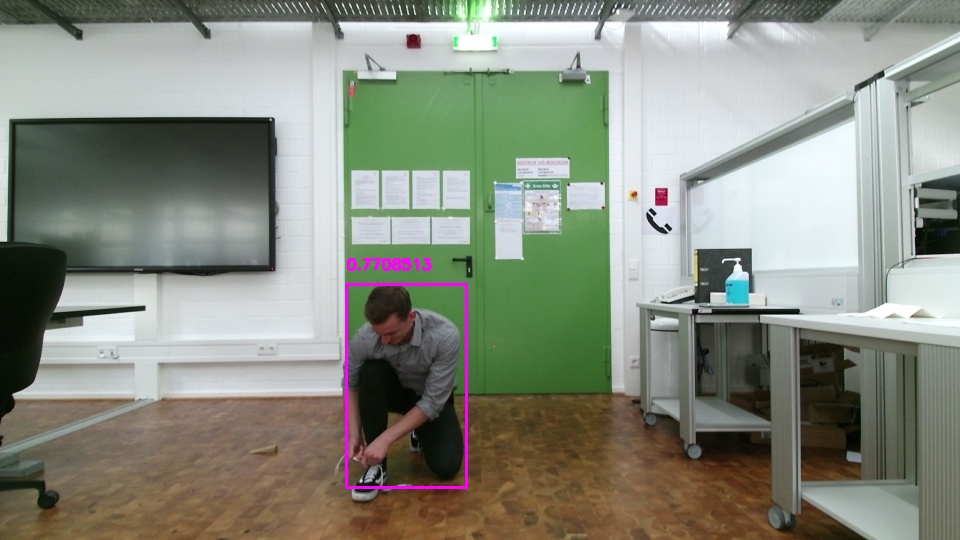
\includegraphics[width=0.88\textwidth]{Bilder/12.jpg}
	\caption{Darstellung einer Person mit kniender Körperhaltung. Die \textit{Bounding Box} des modifizierten \textit{MobileNet V2 SSDLite} ist in pinker Farbe dargestellt.}
	\label{fig: ownnetiou}
\end{figure}
Personen sind auf den Bildern im Trainingsdatensatz häufig sitzend oder stehend abgebildet. Das Netz ist somit nicht darauf trainiert, Personen in anderen Körperhaltungen zu erkennen. Folglich ist eine extrahierte Konfidenz von 77 \% für eine Erkennung einer knienden Person als positiv zu werten. Weiterhin ist die Größe der ausgegebenen \textit{Bounding Box} nahezu gleich gegenüber des grundwahren Begrenzungsrahmens. Der \textit{IoU}-Wert fällt somit deutlich höher aus als der der \textit{HOG-SVM} Kombination.



\subsection{Gegenüberstellung der Objekterkennungssysteme}

Nachfolgend werden die Benchmarkergebnisse der untersuchten Objekterkennungssysteme gegenübergestellt. Der Vergleich dient zur Veranschaulichung der gemessenen \textit{Precision-Recall} Werte je Datensatz.\\

In Abbildung \ref{fig: genauigkeitsvergleich} werden die untersuchten \textit{MobileNet} Architekturen anhand des eigenen Datensatzes verglichen. So kann eine Aussage darüber getroffen werden, ob die Systeme ortsabhängig ein anderes Verhaltensmuster aufzeigen. Es kann beispielsweise vorkommen, dass die Netze aufgrund prägnanter Eigenschaften der Umgebung am Standort der Hochschule Bochum verschieden reagieren.\\


\begin{figure}[H]
	\centering
	\begin{tikzpicture}[
	]
	\begin{axis}[
	width=12cm,
	height=7cm,
	axis y line*=left,
	ticklabel style={% gilt für x und y
		/pgf/number format/.cd,
		use comma,% Komma als Dezimaltrenner
		1000 sep = {}% keine Tausendertrennung 
	},
	xlabel={$\text{Recall } \textit{r(t)}$},
	ylabel={$\text{Precision } \textit{p(t)}$},
	axis x line*=bottom,
	xmin=0.5, xmax=0.9, 
	ymin=0, ymax=1.2,
	%every axis plot/.append style={line width=1.0pt}
	%legend pos=north east,
	legend cell align={left},
	legend style={at={(axis cs:0.75,1)},anchor=south west} ,
	]
	
	\addlegendentry{\footnotesize V2 SSDLite (90)}; % legende1
	\addplot[gray!60, line width=0.8pt]  table [x=Step,y=Value,col sep=comma] from {Bilder/ssdmobilenetv2tflite.csv};
%	\addplot[line width=0.8pt]  table [x=Step,y=Value,col sep=comma] from {Bilder/hog.csv};
	\addplot[dashed,line width=0.8pt]  table [x=Step,y=Value,col sep=comma] from {Bilder/ownnetv2.csv};
	\addplot[gray!60,dashed,line width=0.8pt]  table [x=Step,y=Value,col sep=comma] from {Bilder/ownnetv2ssdlite.csv};
	\addplot[dotted,line width=0.8pt]  table [x=Step,y=Value,col sep=comma] from {Bilder/ownssdmobilenetv1.csv};
	\addplot[dash dot,line width=0.8pt]  table [x=Step,y=Value,col sep=comma] from {Bilder/cocossdmobilenetv1tflite.csv};
	\addlegendimage{/pgfplots/refstyle=plotbrr};				
%	\addlegendentry{HoG \& SVM (H)} ;
	\addlegendentry{\footnotesize mod. V2 SSD (1)} ;%legende 2;
	\addlegendentry{\footnotesize mod. V2 SSDLite (1)} ;%legende 2;
	\addlegendentry{\footnotesize mod. V1 SSD (1)} ;%legende 2;
	\addlegendentry{\footnotesize quant. V1 SSD (90)} ;%legende 2;
	%\addlegendentry{plot 1}
	\end{axis}
	\end{tikzpicture}
	\caption{\textit{Precision-Recall}-Kurven aller Objekterkennungssysteme in Anwendung auf den eigenen Datensatz. Das Kürzel \textit{H} steht für heruntergeladene Systeme und das \textit{E} für entwickelte.}
	\label{fig: genauigkeitsvergleich}

	
\end{figure}


Eine allgemeine Aussage über die Genauigkeiten kann anhand der Darstellung \ref{fig: genauigkeitsvergleichcoco} getroffen werden. Für die Verallgemeinerung sorgt hierbei der \textit{COCO}-Datensatz. Dieser enthält anders als der eigene Datensatz Bilder von verschiedenen Orten.     





\begin{figure}[H]
	\centering
		\begin{tikzpicture}[
	]
	\begin{axis}[
		width=12cm,
		height=7cm,
		axis y line*=left,
		ticklabel style={% gilt für x und y
			/pgf/number format/.cd,
			use comma,% Komma als Dezimaltrenner
			1000 sep = {}% keine Tausendertrennung 
		},
		xlabel={$\text{Recall } \textit{r(t)}$},
		ylabel={$\text{Precision } \textit{p(t)}$},
		axis x line*=bottom,
		xmin=0.0, xmax=0.7, 
		ymin=0, ymax=1.2,
		%every axis plot/.append style={line width=1.0pt}
		%legend pos=north east,
		legend cell align={left},
		legend style={at={(0.5,1)},anchor=north} ,
		legend columns = 3,
		]
		
		\addlegendentry{\scriptsize V2 SSDLite (90)}; % legende1
		\addplot[gray!60, line width=0.8pt]  table [x=Step,y=Value,col sep=comma] from {Bilder/ssdmobilenetv2tflitecoco.csv};
		%	\addplot[line width=0.8pt]  table [x=Step,y=Value,col sep=comma] from {Bilder/hog.csv};
		\addplot[dashed,line width=0.8pt]  table [x=Step,y=Value,col sep=comma] from {Bilder/ownnetv2coco.csv};
		\addplot[gray!60,dashed,line width=0.8pt]  table [x=Step,y=Value,col sep=comma] from {Bilder/ownnetv2ssdlitecoco.csv};
		\addplot[dotted,line width=0.8pt]  table [x=Step,y=Value,col sep=comma] from {Bilder/ownnetv1coco.csv};
		\addplot[dash dot,line width=0.8pt]  table [x=Step,y=Value,col sep=comma] from {Bilder/cocossdmobilenetv1cocotest.csv};
		\addlegendimage{/pgfplots/refstyle=plotbrr};				
		%	\addlegendentry{HoG \& SVM (H)} ;
		\addlegendentry{\scriptsize mod. V2 SSD (1)} ;%legende 2;
		\addlegendentry{\scriptsize mod. V2 SSDLite (1)} ;%legende 2;
		\addlegendentry{\scriptsize mod. V1 SSD (1)} ;%legende 2;
		\addlegendentry{\scriptsize quant. V1 SSD (90)} ;%legende 2;
		%\addlegendentry{plot 1}
	\end{axis}
\end{tikzpicture}
	\caption{\textit{Precision-Recall}-Kurven aller \textit{MobileNet} Netze in Anwendung auf den \textit{COCO}-Datensatz. Die Abkürzungen \textit{mod.} und \textit{quant.} stehen für \textit{modifiziert} und \textit{quantisiert}.}
	\label{fig: genauigkeitsvergleichcoco}
	
	

	
\end{figure}



Bei den Auswertungen der \textit{Precision-Recall} Werte erreichte die Kombination aus \textit{HOG} und \textit{SVM} im Vergleich zu den \textit{MobileNet} Netzen niedrige Ergebnisse. In den Vergleichsgrafiken \ref{fig: genauigkeitsvergleich} und \ref{fig: genauigkeitsvergleichcoco} wird das System aufgrund dessen nicht weiter betrachtet.\\

Überwiegend fällt das quantisierte \textit{MobileNet V1 SSD} Netz in Abbildung \ref{fig: genauigkeitsvergleich} auf. Die Kurve des Netzes verläuft tiefer als die der anderen Architekturen. Das Verhältnis aus \textit{Precision} und \textit{Recall} reduziert sich bei derartigen Strukturen vermutlich durch eine Quantisierung. Netzoptimierungen wie die zweite Version des \textit{MobileNets} oder die Weiterentwicklung des \textit{SSDs} zeigen vorwiegend geringere \textit{Recall}-Werte. Jedoch gibt es im Verlauf der \textit{Precision}-Werte keine nennenswerte Unterschiede. \\

Die Berechnungszeit pro Bild des eigenen Datensatzes aller untersuchten Objekterkennungssysteme ist in Tabelle \ref{fig: zeitentab} präsentiert. Die Tabelle basiert auf der Benchmark, die auf dem Rechner des ALFs in Anwendung auf den eigenen Datensatz durchgeführt wurde.\\

\begin{table}[H]
	\caption{Vergleich der Rechenzeiten pro Bild auf verschiedenen Hardwareplattformen. Die präsentierten Zeiten wurden für alle Analyseschritte addiert und durch die Anzahl aller Bilder geteilt. Ein Analyseschritt bedeutet in diesem Fall die reine Berechnung des Netzes und exkludiert beispielsweise die Zeit für eine Anpassung des Bildes für das entsprechende Netz.  }
	\begin{center}
		\begin{tabular}{|c|c|c|c|c|}
			\hline
			\multicolumn{1}{|c|}{Hardware} & \multicolumn{1}{c|}{Hog \& SVM} & \multicolumn{1}{c|}{SSD MobileNet V1} & \multicolumn{1}{c|}{SSD MobileNet V2} \\ \hline
			Computer ALF	&73.2 	&69 ms		& 600 $\times$ 1000 	 \\
			Grafikkarte			&77.2 	&46		& 	300 $\times$ 300  	 \\
			Raspberry Pi Model B+			&68.0	&59		& 300 $\times$ 300 \\
			
			\hline
		\end{tabular}
	\end{center}

	\label{fig: mobilessdtab}
\end{table}



Bereits aus den beschriebenen Grundlagen aus Abschnitt \ref{subsec: Objekterkennung durch neuronale Netze} geht eine grobe Schätzung der Rechengeschwindigkeiten hervor. Die gezeigten Messergebnisse spiegeln die Erwartungen aus den Grundlagen wider.\\

\begin{table}[H]
	\caption{Gegenüberstellung der errechneten \textit{mean Average Precision}-Werte. Die Hardwareplattformen sind für die Genauigkeit eines Netzes nicht relevant, da diese auf jeder Plattform denselben Wert hat.  }
	\begin{center}
		
		\begin{tabular}{|c|c|c|c|c|}
			\hline
			\multicolumn{1}{|c|}{Objekterkennungssystem} & \multicolumn{1}{c|}{Eigener Datensatz} & \multicolumn{1}{c|}{COCO-Datensatz} \\ \hline
			HOG \& SVM (1)	& 0,16	& 0,07		 \\
			MobileNet V1 SSD quant. (90)			&0,68	&0,46	 	 \\
			MobileNet V1 SSD mod. (1)		&0,79	&0,56	 \\
			MobileNet V2 SSD mod. (1)	&0,78 &0,54  \\
			MobileNet V2 SSDLite (90)			&0,77	& 0,54	 \\
			MobileNet V2 SSDLite mod. (1)			&0,74	&0,47	 \\
			
			\hline
		\end{tabular}
	\end{center}

	\label{fig: genauigkeiten}
\end{table}



Mit 18 ms Rechenzeit und einer mittleren Durchschnittsgenauigkeit am eigenen Datensatz von 0,74 ist das modifizierte \textit{MobileNet V2 SSDLite} Netz das schnellste in der Benchmark. Jedoch ist eine leichte Regression hinsichtlich der Genauigkeit im Vergleich zu den anderen Architekturen in Tabelle \ref{fig: genauigkeiten} zu erkennen.  




\section{Bewertung der Netzarchitekturen}

Für eine vollständige Übersicht der Evaluationsergebnisse aller \textit{MobileNet} Netze ist der Graph in Abbildung \ref{fig: komplettvergleich} gezeigt. Der belegte Speicherplatz durch die Netze wird durch den Durchmesser der grauen Kreise angedeutet. Auf den Achsen des Diagramms ist sowohl die mittlere Durchschnittsgenauigkeit als auch die Rechenzeit angegeben.\\

Im Beispiel der \textit{SSDLite} Modifikation ist zu erkennen, dass die Änderung der Ausgabeschicht den Speicherplatz minimiert. Dies bestätigt die These aus Abschnitt \ref{subsec: Entwickeltes neuronales Netz}.\\

Das quantisierte \textit{MobileNet V1 SSD} Netz weist im Verhältnis zu den anderen Netzen eine langsame Rechenzeit und eine niedrige Genauigkeit auf. Letzteres wird vermutlich durch die Quantisierung verursacht. Der Grund für die langsame Rechenzeit ist vermutlich ein Fehler seitens des \textit{Tensorflow} Frameworks. Nutzer berichten in diversen Foren von langsamen Rechenzeiten nach einer Quantisierung \cite{quant}. \\

Die Benchmark Ergebnisse zeigen einen stärkeren Anstieg der Rechengeschwindigkeit bei der Verwendung des \textit{SSDLite} Klassifikators. Für die modifizierten \textit{MobileNet V2} Netze verkürzt der Wechsel des Klassifikators die Analysezeit um 4 ms. Zwischen den Versionen der \textit{MobileNet} Architekturen ist keine relevante Leistungsänderung für diese Benchmark zu erkennen. Die Reduktion der Parameter zeichnet sich jedoch in der Größe des benötigten Speicherplatzes ab.\\

Die Auswirkung der Größe eines Netzes und des damit verbundenen Rechenaufwands ist in Abbildung \ref{fig: komplettvergleich} zu beobachten. Durch die in Abschnitt \ref{subsec: Entwickeltes neuronales Netz} beschriebene Modifikation der Netze wurde die jeweilige Architektur auf die Anwendung des ALFs angepasst.\\

\begin{figure}[H]
	\centering
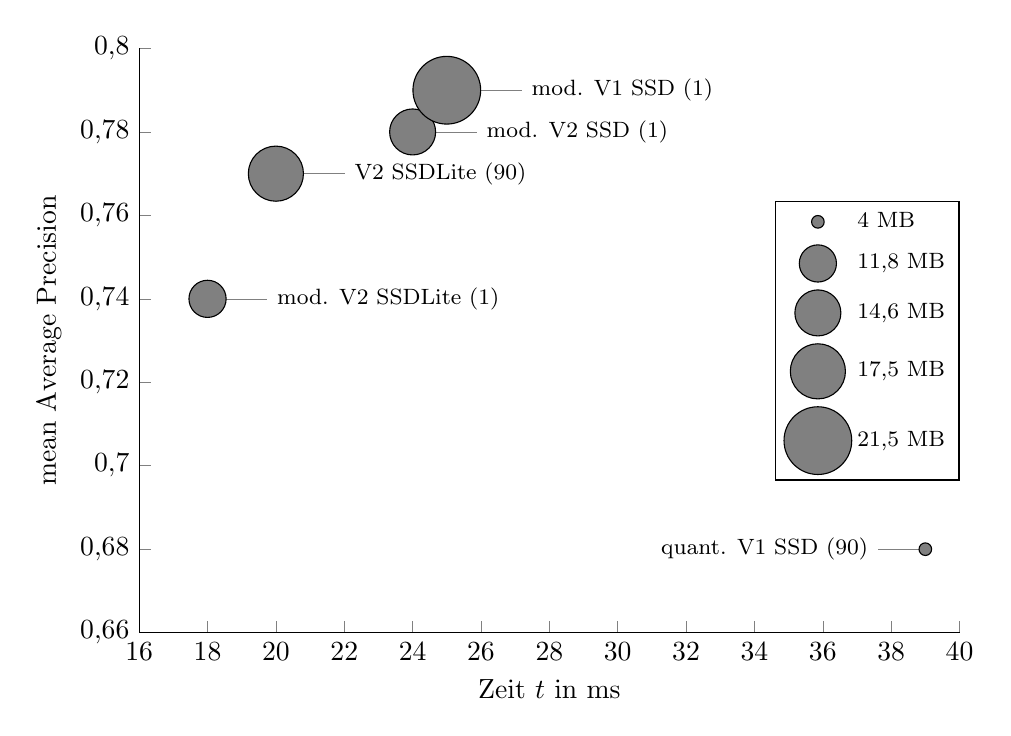
\begin{tikzpicture}
	\begin{axis}[
width=12cm,
height=9cm,
axis y line*=left,
ticklabel style={% gilt für x und y
	/pgf/number format/.cd,
	use comma,% Komma als Dezimaltrenner
	1000 sep = {}% keine Tausendertrennung 
},
xlabel={Zeit $t$ in ms},
ylabel={mean Average Precision},
axis x line*=bottom,
xmin=16, xmax=40, 
ymin=0.66, ymax=0.8,
%every axis plot/.append style={line width=1.0pt}
%legend pos=north east,
legend cell align={left},
legend style={row sep = 0.1cm,at={(1,0.5)},anchor=east} ,
]
\addlegendentry{\footnotesize 4 MB};
\addlegendentry{\footnotesize 11,8 MB};
\addlegendentry{\footnotesize 14,6 MB};
\addlegendentry{\footnotesize 17,5 MB};
\addlegendentry{\footnotesize 21,5 MB};
\addplot[only marks, mark options = {draw =black, scale = 0.04cm, fill = gray}] coordinates{(39,0.68)} node[xshift=0.1cm,pos=0,pin={[pin distance=0.58cm]left:{\footnotesize quant. V1 SSD (90)}}]{} ;
\addplot[only marks, mark options = {draw =black, scale = 0.118cm, fill = gray}] coordinates{(18,0.74)} node[xshift=-0.1cm,pos=0, pin={[pin distance=0.736cm]right:{\footnotesize mod. V2 SSDLite (1)}}]{} ;
\addplot[only marks, mark options = {draw =black, scale = 0.146cm, fill = gray}] coordinates{(24,0.78)} node[xshift=-0.1cm,pos=0, pin={[pin distance=0.792cm]right:{\footnotesize mod. V2 SSD (1)}}]{} ;
\addplot[only marks, mark options = {draw =black, scale = 0.175cm, fill = gray}] coordinates{(20,0.77)} node[xshift=-0.1cm,pos=0, pin={[pin distance=0.85cm]right:{\footnotesize  V2 SSDLite (90)}}]{} ;

\addplot[only marks, mark options = {draw =black, scale = 0.215cm, fill = gray}] coordinates{(25,0.79)} node[xshift=-0.1cm,pos=0, pin={[pin distance=0.93cm]right:{\footnotesize mod. V1 SSD (1)}}]{} ;
\end{axis}
\end{tikzpicture}
	\caption{Vergleich aller untersuchten \textit{MobileNet} Architekturen. Das Diagramm stellt die \textit{mean Average Precision} aufgetragen über die gemessene Rechenzeit dar. Gezeigt ist der Test auf dem integrierten Rechner des ALFs in Anwendung auf den eigenen Datensatz.   }
\label{fig: komplettvergleich}


\end{figure}



Abweichende Werte hinsichtlich der Genauigkeit für gleiche Netzarchitekturen können verschiedene Gründe haben. Der Effekt ist in Abbildung \ref{fig: komplettvergleich} für die \textit{SSDLite} Architekturen zu erkennen. Unter anderem können unterschiedliche Trainingskonfigurationen dazu führen, dass die Genauigkeiten der KNNs abweichen.\\

In Abschnitt \ref{subsec: Eigenschaften von neuronalen Netzen} wurde bereits auf den Einfluss des Trainingsdatensatzes auf das Verhaltensmuster eines Netzes eingegangen. Das große \textit{MobileNet V2 SSDLite} Netz wurde vermutlich nicht mit dem in diesem Projekt verwendeten, benutzerdefinierten \textit{COCO}-Datensatz trainiert. Dies könnte ebenfalls die abweichende Genauigkeit der \textit{SSDLite} Architekturen erklären.\\


Die Abbildungen \ref{fig: owndatat}a und b zeigen erfolgreiche Analysen des modifizierten \textit{MobileNet V2 SSDLite} Netzes. In Abbildung \ref{fig: owndatat}a wurde die linke Person mit einer Konfidenz von 87 \% und die rechte Person mit einer Konfidenz von 67 \% erkannt. Die Darstellung \ref{fig: owndatat}b zeigt, dass die Person im Vordergrund mit einer Wahrscheinlichkeit von 84 \% und die verdeckte Person mit einer Sicherheit von {72~\%} erkannt wurde.  \\

	\begin{figure}[H]
	\centering
	\begin{minipage}[b]{0.49\textwidth}
		(a)
		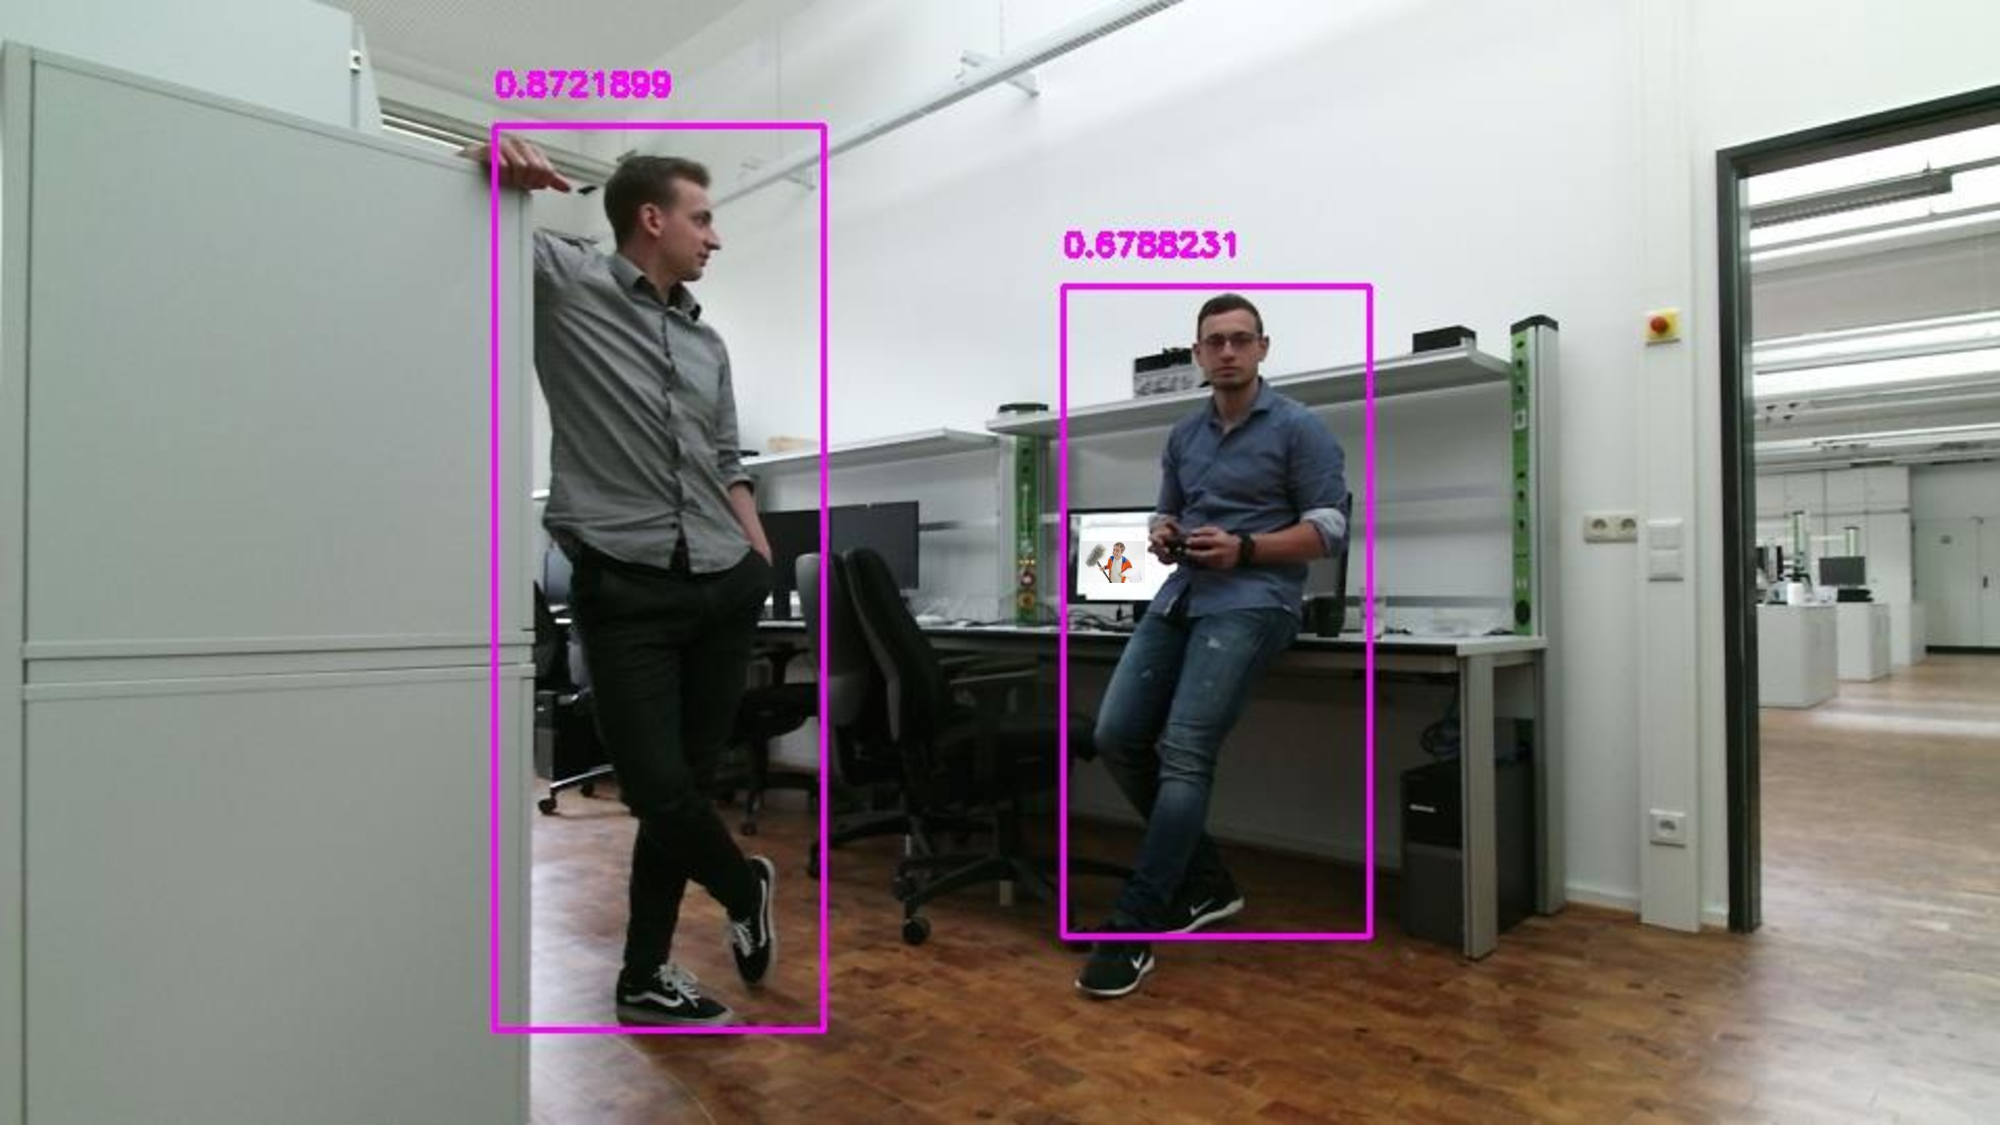
\includegraphics[width=0.94\textwidth]{Bilder/26t.pdf}
	\end{minipage}
	\hfill
	\begin{minipage}[b]{0.49\textwidth}
		(b)
		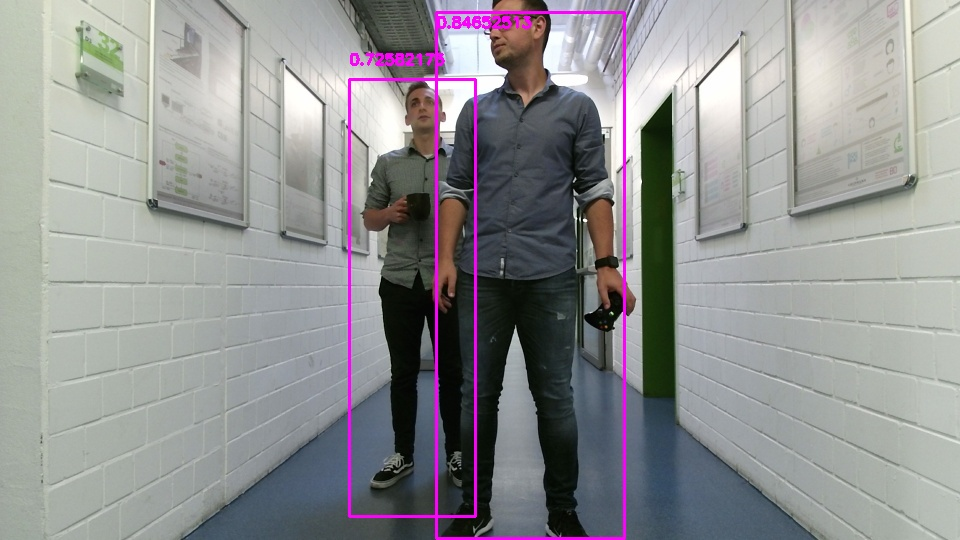
\includegraphics[width=0.94\textwidth]{Bilder/39t.jpg}
	\end{minipage}
	\caption{(a) Foto von zwei Personen im Labor für Antriebstechnik der Hochschule Bochum. Analysiert durch das modifizierte \textit{MobileNet V2 SSDLite} Netz. (b) Darstellung von zwei Menschen. Eine Person ist teilweise verdeckt. Analysiert durch das modifizierte \textit{MobileNet V2 SSDLite} Netz.}
	\label{fig: owndatat}
\end{figure}




Eine fehlerhafte Personenerkennung durch die Kombination aus \textit{HOG} und \textit{SVM} ist in Abbildung \ref{fig: hogtest} dargestellt. Ein Küchentuch wurde fälschlicherweise als Person klassifiziert. Der Grund dafür ist vermutlich die Silhouette des Tuchs.\\

	\begin{figure}[H]
	\centering
	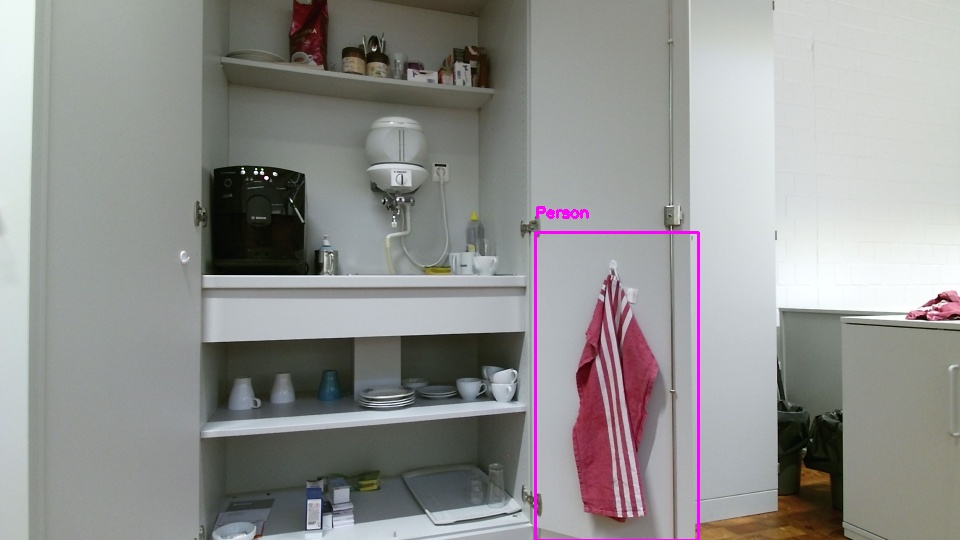
\includegraphics[width=1\textwidth]{Bilder/80.jpg}
	\caption{Veranschaulichung einer fehlerhaften Personenerkennung. Das dargestellte Küchentuch wurde von der \textit{HOG-SVM} Kombination als Person klassifiziert.}
	\label{fig: hogtest}
\end{figure}

 Diese ähnelt grob dem Körperbau eines Menschen. Dies könnte zu einer ähnlichen Struktur, der durch den \textit{HOG} extrahierten Gradienten und somit zu einer fehlerhaften Klassifizierung geführt haben.\\





In diesem Kapitel wurden Objekterkennungssysteme nach verschiedenen Eigenschaften untersucht. Zusammenfassend können zwei der sechs präsentierten Methoden für den Einsatz am ALF sowie auf einem eingebetteten System empfohlen werden. Die Empfehlungen basiert hierbei auf die Berücksichtigung aller dargestellten Messergebnisse und dem jeweiligen Anwendungsfall.\\

Für eine reine Personenerkennung im Nahbereich des Fahrzeugs wird der Einsatz des modifizierten \textit{MobileNet V2 SSDLite} empfohlen. Das Netz erreicht sowohl auf dem Computer des ALFs als auch auf dem \textit{Raspberry Pi} die geringsten Analysezeiten. Lässt der Anwendungsfall eine Genauigkeit von 0,74 zu, ist die genannte Architektur zu wählen.\\

Die Rechenzeit der großen \textit{MobileNet V2 SSDLite} Architektur ist lediglich 2 ms langsamer als das modifizierte Netz. Somit lassen sich mit nahezu gleicher Geschwindigkeit deutlich mehr Objekte erkennen. Wenn es folglich um die Erkennung mehrerer Klassen geht, wird die Implementierung des \textit{MobileNet V2 SSDLite} Netzes mit 90 Klassen empfohlen.\\ 